\chapter{Design}
% Design dell'architettura del sistema e delle interfacce utente.

\section{Frontend}

% https://www.usability.gov/what-and-why/user-centered-design.html#:~:text=The%20User%2Dcentered%20design%20(UCD,basis%20for%20many%20UCD%20methodologies.

% https://www.interaction-design.org/literature/topics/personas#:~:text=Personas%20are%20fictional%20characters%2C%20which,%2C%20experiences%2C%20behaviors%20and%20goals.

Ascent Essentials è un E-Commerce specializzato rivolto agli appassionati di attività sportive in montagna, quindi l'interfaccia utente è stata progettata con attenzione per riflettere la natura avventurosa e dinamica della clientela.

Lo \textit{User-Centered Design} fa parte della filosofia di Ascent Essentials. Ogni aspetto dell'interfaccia e dell'esperienza utente è stato progettato con l'obiettivo di soddisfare le esigenze e le aspettative degli appassionati di attività sportive in montagna:

\begin{itemize}
    \item \textbf{Ricerca utente approfondita}: Prima di iniziare il processo di progettazione, è stata condotta una ricerca approfondita sugli utenti target, compresi gli appassionati di arrampicata, alpinismo e trekking. Sono state utilizzate tecniche come interviste, sondaggi e analisi dei dati per comprendere le esigenze, i comportamenti e le preferenze degli utenti.
    \item \textbf{Coinvolgimento attivo degli utenti}: Gli utenti sono stati coinvolti attivamente durante tutto il processo di progettazione attraverso sessioni di feedback e test utente.
    \item \textbf{Creazione di Personas}: Sono state create Personas rappresentative degli utenti target (come Luca l'Alpinista e Sofia la Trekker) per focalizzare la progettazione su utenti specifici con esigenze e obiettivi distinti. Le Personas sono diventate guide chiave per valutare ogni aspetto del design, assicurando che soddisfi le esigenze di utenti reali.
    \item \textbf{Test iterativi}: L'approccio di progettazione ha incorporato cicli iterativi di test utente per identificare e correggere rapidamente eventuali problemi o inefficienze nell'interfaccia utente. Ogni fase del design è stata seguita da test utente, permettendo un'evoluzione continua basata sul feedback reale.
    \item \textbf{Design responsivo}: L'interfaccia è stata progettata per essere totalmente responsiva, garantendo un'esperienza utente coerente su diverse piattaforme e dispositivi. L'utilizzo di design fluido e layout adattivi assicura che Ascent Essentials sia accessibile su dispositivi mobili, tablet e desktop.
    \item \textbf{Accessibilità universale}: L'attenzione è stata posta sulla progettazione di un'interfaccia accessibile, rispettando le linee guida WCAG per garantire che tutti gli utenti, indipendentemente dalle loro capacità, possano utilizzare l'applicazione. Test automatici e manuali sono stati eseguiti per assicurare che l'applicazione rispetti gli standard di accessibilità.
    \item \textbf{Approccio empatico}: Gli sviluppatori hanno adottato un approccio empatico, cercando di comprendere le emozioni e le prospettive degli utenti per migliorare la qualità dell'esperienza utente complessiva. Le decisioni di design sono state guidate non solo da dati oggettivi, ma anche da una comprensione empatetica delle esigenze e dei desideri degli utenti.
\end{itemize}

\subsection{Personas}

\textbf{Persona 1: Luca l'Alpinista}

\textbf{Demografia:}
\begin{itemize}
    \item Età: 35 anni
    \item Occupazione: Insegnante di arrampicata professionista
    \item Posizione: Trento, Italia
\end{itemize}

\textbf{Caratteristiche:}
\begin{itemize}
    \item Luca è un alpinista esperto e appassionato che trascorre la maggior parte del suo tempo in montagna.
    \item Cerca attrezzature tecniche di alta qualità per affrontare le sfide dell'alpinismo.
    \item Desidera ricevere consigli da esperti e leggere recensioni dettagliate prima di acquistare.
\end{itemize}

\textbf{Obiettivi:}
\begin{itemize}
    \item Trovare attrezzature tecniche specifiche per le sue scalate.
    \item Ricevere consigli da esperti sulla giusta attrezzatura.
    \item Essere ispirato da racconti di avventure simili.

\end{itemize}

\textbf{Persona 2: Sofia la Trekker}

\textbf{Demografia:}
\begin{itemize}
    \item Età: 28 anni
    \item Occupazione: Fotografa naturalistica
    \item Posizione: Barcellona, Spagna
\end{itemize}

\textbf{Caratteristiche:}
\begin{itemize}
    \item Sofia è una trekker appassionata che ama esplorare nuovi sentieri e paesaggi naturali.
    \item Cerca attrezzature leggere e funzionali per rendere più piacevoli le sue escursioni.
    \item Desidera condividere le sue esperienze con una comunità di appassionati.
\end{itemize}

\textbf{Obiettivi:}
\begin{itemize}
    \item Esplorare facilmente una vasta gamma di prodotti adatti al trekking.
    \item Ricevere consigli su accessori pratici e leggeri.
    \item Condividere esperienze e consigli con altri appassionati.

\end{itemize}

\textbf{Persona 3: Elena la Principiante}

\textbf{Demografia:}
\begin{itemize}
    \item Età: 24 anni
    \item Occupazione: Studentessa universitaria
    \item Posizione: Firenze, Italia
\end{itemize}

\textbf{Caratteristiche:}
\begin{itemize}
    \item Elena è nuova nell'alpinismo e cerca attrezzature di qualità adatte ai principianti.
    \item Ha un budget limitato ma desidera investire in prodotti duraturi.
    \item Cerca un'esperienza di acquisto intuitiva e facile.
\end{itemize}

\textbf{Obiettivi:}
\begin{itemize}
    \item Trovare attrezzature adatte ai principianti.
    \item Risparmiare senza compromettere la qualità.
    \item Apprendere più cose sull'alpinismo attraverso l'accesso a risorse educative.

\end{itemize}

\textbf{Persona 4: Marco l'Appassionato di Escursioni}

\textbf{Demografia:}
\begin{itemize}
    \item Età: 40 anni
    \item Occupazione: Manager aziendale
    \item Posizione: Monaco di Baviera, Germania
\end{itemize}

\textbf{Caratteristiche:}
\begin{itemize}
    \item Marco è un appassionato di escursioni che ama trascorrere il tempo libero nella natura.
    \item Cerca prodotti affidabili e versatili che si adattino a diverse attività all'aperto.
    \item Desidera una piattaforma intuitiva per esplorare rapidamente nuovi arrivi e offerte speciali.
\end{itemize}

\textbf{Obiettivi:}
\begin{itemize}
    \item Trovare attrezzature versatili per diverse attività all'aperto.
    \item Essere aggiornato sulle nuove offerte e sconti.
    \item Esplorare prodotti in modo rapido ed efficiente.
\end{itemize}

\subsection{Interfaccia Utente}

In Figura \ref{fig:site-map} viene presentata la mappa dei componenti dell'interfaccia grafica:

\begin{itemize}
    \item \textbf{Cart (Carrello):} Rappresenta il carrello dell'utente.
    \item \textbf{CategoriesManagement (Gestione Categorie):} Gestisce le categorie di prodotti.
    \item \textbf{CategoryProducts (Prodotti per Categoria):} Rappresenta i prodotti all'interno di una categoria specifica.
    \item \textbf{Checkout (Pagamento):} Gestisce il processo di pagamento e checkout.
    \item \textbf{CouponsManagement (Gestione Coupon):} Gestisce i coupon.
    \item \textbf{CustomerAccount (Account Cliente):} Rappresenta l'account di un cliente.
    \item \textbf{Header:} È il coponente in testa a tutte le pagine ed associato a diverse funzionalità come Notifiche, Account Utente, Carrello, Ricerca Prodotti, etc.
    \item \textbf{Home (Pagina Principale):} Rappresenta la pagina principale.
    \item \textbf{NewProduct (Nuovo Prodotto):} Rappresenta la funzionalità per aggiungere nuovi prodotti.
    \item \textbf{Notifications (Notifiche):} Gestisce le notifiche per gli utenti.
    \item \textbf{OrdersManagement (Gestione Ordini):} Gestisce gli ordini effettuati dagli utenti.
    \item \textbf{Product (Prodotto):} Rappresenta un singolo prodotto.
    \item \textbf{ProductsManagement (Gestione Prodotti):} Gestisce l'inventario e le informazioni sui prodotti.
    \item \textbf{SearchProducts (Ricerca Prodotti):} Rappresenta la funzionalità di ricerca dei prodotti.
    \item \textbf{SupplierAccount (Account Fornitore):} Rappresenta l'account di un fornitore.
    \item \textbf{UserAccount (Account Utente):} È un'astrazione generale dell'account utente, che può essere specializzato in CustomerAccount o SupplierAccount.
    \item \textbf{UserLogin (Accesso Utente):} Gestisce il processo di accesso e autenticazione degli utenti.
\end{itemize}

\begin{figure}
    \centering
    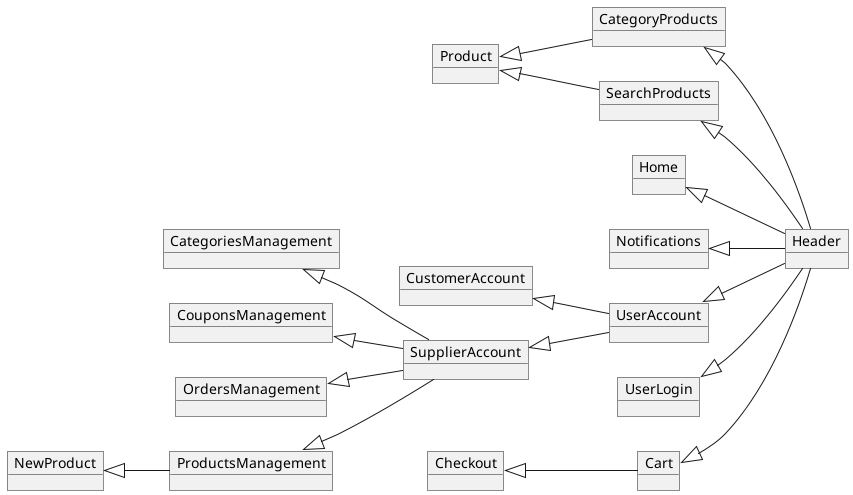
\includegraphics[width=0.8\textwidth]{figures/site-map.png}
    \caption{Mappa dei componenti dell'interfaccia grafica}
    \label{fig:site-map}
\end{figure}

\section{Backend}
Il backend dell'E-commerce è progettato seguendo un'architettura RESTful con operazioni CRUD.

\subsection{Struttura delle Classi}
\begin{itemize}
    \item \textbf{Classi Model:} Utilizzate per definire la struttura e i campi delle entità del sistema.
    \item \textbf{Classi Route:} Definiscono le rotte dell'API. Ogni classe route contiene un gruppo di rotte correlate.
    \item \textbf{Classi Controller:} Utilizzate per gestire le richieste. Ogni classe controller contiene un gruppo di metodi che gestiscono le richieste.
    \item \textbf{Middleware:} I middleware vengono eseguiti prima di ogni richiesta HTTP. Sono utilizzati per gestire l'autenticazione e l'autorizzazione.
\end{itemize}

\subsection{Documentazione dell'API}
La documentazione dell'API è realizzata utilizzando Swagger con la specifica OpenAPI. Questo strumento semplifica la comprensione e l'utilizzo delle risorse messe a disposizione dal backend. L'interfaccia Swagger è accessibile solamente in fase di sviluppo, in quanto non è necessaria in produzione.
Di seguito vengono indicate le rotte disponibili:

\subsubsection{Cart endpoints:}
\begin{itemize}
    \item \textbf{GET /cart} - Restituisce il carrello dell'utente.
    \item \textbf{POST /cart/add} - Aggiunge un prodotto al carrello dell'utente.
    \item \textbf{PUT /cart/update} - Aggiorna la quantità di un prodotto nel carrello dell'utente.
    \item \textbf{DELETE /cart/remove} - Rimuove un prodotto dal carrello dell'utente.
    \item \textbf{DELETE /cart/clear} - Svuota il carrello dell'utente.
\end{itemize}

\subsubsection{Category endpoints:}
\begin{itemize}
    \item \textbf{GET /categories} - Restituisce tutte le categorie.
    \item \textbf{GET /category} - Restituisce una categoria.
    \item \textbf{POST /category} - Crea una nuova categoria.
    \item \textbf{GET /subcategories} - Restituisce tutte le sottocategorie.
    \item \textbf{GET /subcategory} - Restituisce una sottocategoria.
    \item \textbf{POST /subcategory} - Crea una nuova sottocategoria.
    \item \textbf{PUT /subcategory/\{id\}} - Aggiorna una sottocategoria.
\end{itemize}

\subsubsection{Coupons endpoints:}
\begin{itemize}
    \item \textbf{GET /admin/coupons} - Restituisce tutti i coupon.
    \item \textbf{POST /admin/coupon} - Crea un nuovo coupon.
    \item \textbf{GET /coupon/\{code\}} - Restituisce un coupon.
    \item \textbf{DELETE /admin/coupon/\{code\}} - Rimuove un coupon.
    \item \textbf{PATCH /admin/coupon/\{code\}} - Aggiorna lo sconto di un coupon.
\end{itemize}

\subsubsection{Notification endpoints:}
\begin{itemize}
    \item \textbf{GET /notifications} - Restituisce tutte le notifiche dell'utente.
    \item \textbf{GET /admin/notifications} - Restituisce le notifiche per gli amministratori.
    \item \textbf{DELETE /notification/\{notificationId\}} - Rimuove una notifica.
    \item \textbf{DELETE /admin/notification/\{notificationId\}} - Rimuove una notifica per gli amministratori.
\end{itemize}

\subsubsection{Order endpoints:}
\begin{itemize}
    \item \textbf{GET /orders} - Restituisce tutti gli ordini dell'utente.
    \item \textbf{GET /orders/\{orderId\}} - Restituisce un ordine.
    \item \textbf{GET /admin/orders} - Restituisce tutti gli ordini.
    \item \textbf{POST /order} - Crea un nuovo ordine.
    \item \textbf{GET /admin/orders/user/\{userId\}} - Restituisce tutti gli ordini di un utente.
    \item \textbf{PATCH /admin/orders/\{orderId\}/status} - Aggiorna lo stato di un ordine.
    \item \textbf{DELETE /admin/orders/\{orderId\}} - Rimuove un ordine.
\end{itemize}

\subsubsection{Product endpoints:}
\begin{itemize}
    \item \textbf{POST /product} - Crea un nuovo prodotto.
    \item \textbf{GET /product/image/\{imageName\}} - Serve un'immagine specifica del prodotto.
    \item \textbf{GET /products} - Ottieni tutti i prodotti.
    \item \textbf{GET /products/category/\{categoryId\}} - Ottieni tutti i prodotti in una categoria.
    \item \textbf{GET /products/subcategory/\{subcategoryId\}} - Ottieni tutti i prodotti di una sottocategoria.
    \item \textbf{GET /product/\{productId\}} - Ottieni un prodotto per ID.
    \item \textbf{PUT /product/\{productId\}} - Aggiorna i dettagli di un prodotto.
    \item \textbf{DELETE /product/\{productId\}} - Elimina un prodotto per ID.
    \item \textbf{GET /products/search} - Cerca prodotti in base a una stringa di query.
\end{itemize}

\subsubsection{User endpoints:}
\begin{itemize}
    \item \textbf{POST /register} - Registra un nuovo utente.
    \item \textbf{POST /login} - Effettua l'accesso come utente.
    \item \textbf{GET /user} - Ottieni i dettagli dell'utente.
\end{itemize}

\subsection{Sicurezza e Autenticazione}
Per garantire la sicurezza del sistema, è stato implementato un sistema di autenticazione basato su JSON Web Tokens (JWT). Le password degli utenti sono crittografate utilizzando l'algoritmo bcrypt, garantendo un'adeguata sicurezza delle credenziali. Questo approccio offre vantaggi in termini di sicurezza e scalabilità.


\section{Database}
Per gestire la persistenza dei dati, è stato adottato MongoDB come sistema di database, utilizzando la libreria Mongoose per semplificare l'interazione con il database NoSQL.

Il database è stato progettato seguendo uno schema che riflette la struttura delle entità nel sistema.
Le entità presenti nel database sono le seguenti:
\begin{itemize}
    \item \textbf{Cart:} Rappresenta il carrello di un utente.
    \item \textbf{Category:} Rappresenta una categoria di prodotti.
    \item \textbf{Coupon:} Rappresenta un coupon.
    \item \textbf{Notification:} Rappresenta una notifica.
    \item \textbf{Order:} Rappresenta un ordine.
    \item \textbf{Product:} Rappresenta un prodotto.
    \item \textbf{Subcategory:} Rappresenta una sottocategoria di prodotti.
    \item \textbf{User:} Rappresenta un utente.
\end{itemize}

Sono stati implementati indici su specifici campi al fine di ottimizzare le query e potenziare le prestazioni del database. Inoltre, sono state instaurate relazioni tra le diverse entità per agevolare l'accesso ai dati correlati. Un esempio di ciò è la correlazione tra un prodotto e una sottocategoria, semplificando notevolmente l'accesso alle informazioni pertinenti.

In aggiunta, alcuni schemi sono stati definiti con validazioni personalizzate per garantire la coerenza dei dati, come ad esempio l'assicurarsi che le sottocategorie e i prodotti referenziati siano validi.

Laddove necessario, sono stati impiegati timestamp automatici per registrare la data di creazione e gli eventuali aggiornamenti di un documento.
